\documentclass[12pt]{article}
\usepackage{setspace}  % To use linespacing
\usepackage{indentfirst} % Indents first line after sections
\usepackage{amssymb} % For \mathbb
\usepackage{enumerate} % For changing labels of enumerate
\usepackage[margin=1in]{geometry} % For editing margins
\usepackage{tikz} % Tikz drawing for graphs
\usetikzlibrary{arrows.meta} % Allows customizing arrows
\usetikzlibrary{backgrounds} % For framing a tikzpicture
\usetikzlibrary{calc, through}
\usetikzlibrary{decorations.markings}
\usetikzlibrary{arrows}
\usetikzlibrary{positioning}
\usepackage{amsmath}
\usepackage{ifthen}
\usepackage{intcalc} % \intcalcMod

% Make new commands
\newcommand{\N}{\mathbb{N}}
\newcommand{\R}{\mathbb{R}}
\newcommand{\Z}{\mathbb{Z}}
\newcommand{\abs}[1]{\left|#1\right|}
\newcommand{\paren}[1]{\left(#1\right)}
\newcommand{\fivespace}{\space\space\space\space\space}

\newcommand{\be}{\begin{enumerate}}
\newcommand{\ee}{\end{enumerate}}
\newcommand{\seti}[1]{\setcounter{enumi}{#1}}
\newcommand{\setii}[1]{\setcounter{enumii}{#1}}

% Start main document
\begin{document}
\onehalfspacing
\hfill Frank Cline

\hfill Math 307

\hfill HW 9

% PROBLEMS
\section*{Problems 1-7}

\be
% 1
\item Find the chromatic number  $\chi(G)$ of each of the graphs shown in Figure 1. To do so: (1) provide a coloring (with actual colors) for each of the graphs using $\chi(G)$ colors, and (2) explain why you cannot use fewer colors.
	\be
	% 1 a
	\item $\chi(G)=4$. The outer vertices creates an odd cycle, so there must be at least 3 colorings, and the center vertices 
	connects to all the vertices, so it must be colored differently. That gives us $3+1$ colorings which is 4.\vspace{0.5cm}\\
	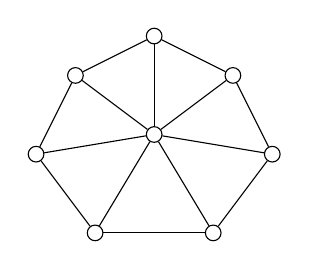
\begin{tikzpicture}
	\begin{scope}[every node/.style={circle, draw, inner sep = 2pt}]
	    	\node (1) at (0,0) {};
		\node (2) at (1,-0.5) {};
	    	\node (3) at (1.5,-1.5) {};
		\node (4) at (0.75,-2.5) {};
	    	\node (5) at (-0.75,-2.5) {};
	    	\node (6) at (-1.5,-1.5) {};
		\node (7) at (-1,-0.5) {};
	    	\node (8) at (0,-1.25) {};
	\end{scope}
	
	\begin{scope}[>={Stealth[black]},
	              every node/.style={fill=white,circle},
	              every edge/.style={draw=black}]
		\path (1) edge (2);
		\path (2) edge (3);
		\path (3) edge (4);
		\path (4) edge (5);
		\path (5) edge (6);
		\path (6) edge (7);
		\path (7) edge (1);
		\foreach \i in {1,2,3,4,5,6,7}
		{\path (8) edge (\i);}
	\end{scope}
	\end{tikzpicture}
	\hspace{3cm}
	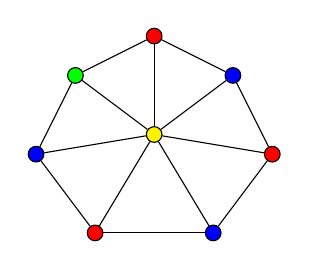
\begin{tikzpicture}
	\begin{scope}[every node/.style={circle, draw, inner sep = 2pt}]
	    	\node[fill=red] (1) at (0,0) {};
		\node[fill=blue] (2) at (1,-0.5) {};
	    	\node[fill=red] (3) at (1.5,-1.5) {};
		\node[fill=blue] (4) at (0.75,-2.5) {};
	    	\node[fill=red] (5) at (-0.75,-2.5) {};
	    	\node[fill=blue] (6) at (-1.5,-1.5) {};
		\node[fill=green] (7) at (-1,-0.5) {};
	    	\node[fill=yellow] (8) at (0,-1.25) {};
	\end{scope}
	
	\begin{scope}[>={Stealth[black]},
	              every node/.style={fill=white,circle},
	              every edge/.style={draw=black}]
		\path (1) edge (2);
		\path (2) edge (3);
		\path (3) edge (4);
		\path (4) edge (5);
		\path (5) edge (6);
		\path (6) edge (7);
		\path (7) edge (1);
		\foreach \i in {1,2,3,4,5,6,7}
		{\path (8) edge (\i);}
	\end{scope}
	\end{tikzpicture}
	
	% 1 b
	\item $\chi(G)=2$. It's two because that is the smallest possible chromatic numbering for a connected graph. \vspace{0.5cm}\\
	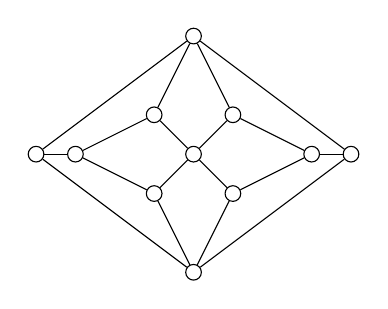
\begin{tikzpicture}[every node/.style={circle, draw, inner sep = 2pt}]
	\begin{scope}[every node/.style={circle, draw, inner sep = 2pt}]
	    	\node (1) at (0,0.5) {};
		\node (2) at (2,-1) {};
	    	\node (3) at (0,-2.5) {};
		\node (4) at (-2,-1) {};
	    	\node (5) at (-1.5,-1) {};
	    	\node (6) at (-0.5,-0.5) {};
		\node (7) at (0.5,-0.5) {};
	    	\node (8) at (1.5,-1) {};
	    	\node (9) at (0.5,-1.5) {};
	    	\node (10) at (-0.5,-1.5) {};
	    	\node (11) at (0,-1) {};
	\end{scope}
	
	\begin{scope}[>={Stealth[black]},
	              every node/.style={fill=white,circle},
	              every edge/.style={draw=black}]
		\path (1) edge (2);
		\path (1) edge (6);
		\path (1) edge (7);
		\path (1) edge (4);
		\path (2) edge (3);
		\path (2) edge (8);
		\path (3) edge (4);
		\path (3) edge (9);
		\path (3) edge (10);
		\path (4) edge (5);
		\path (5) edge (6);
		\path (5) edge (10);
		\path (6) edge (11);
		\path (7) edge (8);
		\path (7) edge (11);
		\path (8) edge (9);
		\path (9) edge (11);
		\path (10) edge (11);
	\end{scope}
	\end{tikzpicture}
	\hspace{2cm}
	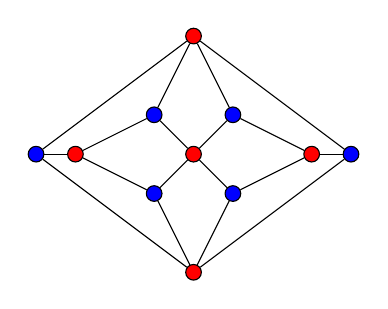
\begin{tikzpicture}[every node/.style={circle, draw, inner sep = 2pt}]
	\begin{scope}[every node/.style={circle, draw, inner sep = 2pt}]
	    	\node[fill=red] (1) at (0,0.5) {};
		\node[fill=blue] (2) at (2,-1) {};
	    	\node[fill=red] (3) at (0,-2.5) {};
		\node[fill=blue] (4) at (-2,-1) {};
	    	\node[fill=red] (5) at (-1.5,-1) {};
	    	\node[fill=blue] (6) at (-0.5,-0.5) {};
		\node[fill=blue] (7) at (0.5,-0.5) {};
	    	\node[fill=red] (8) at (1.5,-1) {};
	    	\node[fill=blue] (9) at (0.5,-1.5) {};
	    	\node[fill=blue] (10) at (-0.5,-1.5) {};
	    	\node[fill=red] (11) at (0,-1) {};
	\end{scope}
	
	\begin{scope}[>={Stealth[black]},
	              every node/.style={fill=white,circle},
	              every edge/.style={draw=black}]
		\path (1) edge (2);
		\path (1) edge (6);
		\path (1) edge (7);
		\path (1) edge (4);
		\path (2) edge (3);
		\path (2) edge (8);
		\path (3) edge (4);
		\path (3) edge (9);
		\path (3) edge (10);
		\path (4) edge (5);
		\path (5) edge (6);
		\path (5) edge (10);
		\path (6) edge (11);
		\path (7) edge (8);
		\path (7) edge (11);
		\path (8) edge (9);
		\path (9) edge (11);
		\path (10) edge (11);
	\end{scope}
	\end{tikzpicture}
	
	% 1 c
	\item $\chi(G)=3$. It's three because there contains an odd cycle, so the chromatic number must be at least 3. \vspace{0.5cm}		\\
	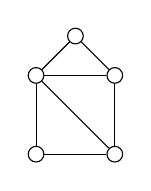
\begin{tikzpicture}
	\begin{scope}[every node/.style={circle, draw, inner sep = 2pt}]
	    	\node (1) at (0,0) {};
		\node (2) at (0,1) {};
	    	\node (3) at (0.5,1.5) {};
		\node (4) at (1,1) {};
	    	\node (5) at (1,0) {};
	\end{scope}
	
	\begin{scope}[>={Stealth[black]},
	              every node/.style={fill=white,circle},
	              every edge/.style={draw=black}]
		\path (1) edge (2);
		\path (1) edge (5);
		\path (2) edge (3);
		\path (2) edge (4);
		\path (2) edge (5);
		\path (3) edge (4);
		\path (4) edge (5);
	\end{scope}
	\end{tikzpicture}
	\hspace{2cm}
	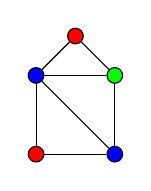
\begin{tikzpicture}
	\begin{scope}[every node/.style={circle, draw, inner sep = 2pt}]
	    	\node[fill=red] (1) at (0,0) {};
		\node[fill=blue] (2) at (0,1) {};
	    	\node[fill=red] (3) at (0.5,1.5) {};
		\node[fill=green] (4) at (1,1) {};
	    	\node[fill=blue] (5) at (1,0) {};
	\end{scope}
	
	\begin{scope}[>={Stealth[black]},
	              every node/.style={fill=white,circle},
	              every edge/.style={draw=black}]
		\path (1) edge (2);
		\path (1) edge (5);
		\path (2) edge (3);
		\path (2) edge (4);
		\path (2) edge (5);
		\path (3) edge (4);
		\path (4) edge (5);
	\end{scope}
	\end{tikzpicture}

	% 1 d
	\item $\chi(G)=4$. It's four because there contains an odd cycle, so the chromatic number must be at least 3. There is also a 
	vertex that connects to all other vertices, so for it's color to be different there must be $3+1$ colorings which is 4. 
	\vspace{0.5cm}\\
	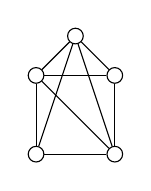
\begin{tikzpicture}
	\begin{scope}[every node/.style={circle, draw, inner sep = 2pt}]
	    	\node (1) at (0,0) {};
		\node (2) at (0,1) {};
	    	\node (3) at (0.5,1.5) {};
		\node (4) at (1,1) {};
	    	\node (5) at (1,0) {};
	\end{scope}
	
	\begin{scope}[>={Stealth[black]},
	              every node/.style={fill=white,circle},
	              every edge/.style={draw=black}]
		\path (1) edge (2);
		\path (1) edge (5);
		\path (1) edge (3);
		\path (2) edge (3);
		\path (2) edge (4);
		\path (2) edge (5);
		\path (3) edge (4);
		\path (3) edge (5);
		\path (4) edge (5);
	\end{scope}
	\end{tikzpicture}
	\hspace{2cm}
	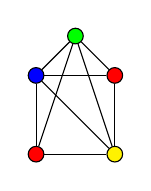
\begin{tikzpicture}
	\begin{scope}[every node/.style={circle, draw, inner sep = 2pt}]
	    	\node[fill=red] (1) at (0,0) {};
		\node[fill=blue] (2) at (0,1) {};
	    	\node[fill=green] (3) at (0.5,1.5) {};
		\node[fill=red] (4) at (1,1) {};
	    	\node[fill=yellow] (5) at (1,0) {};
	\end{scope}
	
	\begin{scope}[>={Stealth[black]},
	              every node/.style={fill=white,circle},
	              every edge/.style={draw=black}]
		\path (1) edge (2);
		\path (1) edge (5);
		\path (1) edge (3);
		\path (2) edge (3);
		\path (2) edge (4);
		\path (2) edge (5);
		\path (3) edge (4);
		\path (3) edge (5);
		\path (4) edge (5);
	\end{scope}
	\end{tikzpicture}
	
	% 1 e
	\item $\chi(G)=4$. WRITE DOWN WHY HERE!!! \vspace{0.5cm}\\
	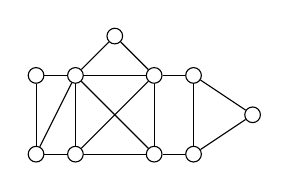
\begin{tikzpicture}
	\begin{scope}[every node/.style={circle, draw, inner sep = 2pt}]
	    	\node (1) at (0,0) {};
		\node (2) at (0,1) {};
	    	\node (3) at (0.5,1) {};
		\node (4) at (1,1.5) {};
	    	\node (5) at (1.5,1) {};
	    	\node (6) at (2,1) {};
	    	\node (7) at (2.75,0.5) {};
	    	\node (8) at (2,0) {};
	    	\node (9) at (1.5,0) {};
	    	\node (10) at (0.5,0) {};
	\end{scope}
	
	\begin{scope}[>={Stealth[black]},
	              every node/.style={fill=white,circle},
	              every edge/.style={draw=black}]
		\path (1) edge (2);
		\path (1) edge (3);
		\path (1) edge (10);
		\path (2) edge (3);
		\path (3) edge (4);
		\path (3) edge (5);
		\path (3) edge (9);
		\path (3) edge (10);
		\path (4) edge (5);
		\path (5) edge (6);
		\path (5) edge (9);
		\path (5) edge (10);
		\path (6) edge (7);
		\path (6) edge (8);
		\path (7) edge (8);
		\path (8) edge (9);
		\path (9) edge (10);
	\end{scope}
	\end{tikzpicture}
	\hspace{2cm}
	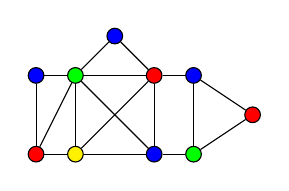
\begin{tikzpicture}
	\begin{scope}[every node/.style={circle, draw, inner sep = 2pt}]
	    	\node[fill=red] (1) at (0,0) {};
		\node[fill=blue] (2) at (0,1) {};
	    	\node[fill=green] (3) at (0.5,1) {};
		\node[fill=blue] (4) at (1,1.5) {};
	    	\node[fill=red] (5) at (1.5,1) {};
	    	\node[fill=blue] (6) at (2,1) {};
	    	\node[fill=red] (7) at (2.75,0.5) {};
	    	\node[fill=green] (8) at (2,0) {};
	    	\node[fill=blue] (9) at (1.5,0) {};
	    	\node[fill=yellow] (10) at (0.5,0) {};
	\end{scope}
	
	\begin{scope}[>={Stealth[black]},
	              every node/.style={fill=white,circle},
	              every edge/.style={draw=black}]
		\path (1) edge (2);
		\path (1) edge (3);
		\path (1) edge (10);
		\path (2) edge (3);
		\path (3) edge (4);
		\path (3) edge (5);
		\path (3) edge (9);
		\path (3) edge (10);
		\path (4) edge (5);
		\path (5) edge (6);
		\path (5) edge (9);
		\path (5) edge (10);
		\path (6) edge (7);
		\path (6) edge (8);
		\path (7) edge (8);
		\path (8) edge (9);
		\path (9) edge (10);
	\end{scope}
	\end{tikzpicture}
	\ee

% 2
\item Give examples of a graph (that are not examples from class or the worksheet) for which 
	\be
	% 2 a
	\item $\chi(G)  = \Delta(G)$\\
	$\chi(G)=2$ and $\Delta(G)=2$ and $2=2$. \vspace{0.5cm}\\
	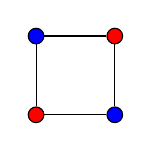
\begin{tikzpicture}
	\begin{scope}[every node/.style={circle, draw, inner sep = 2pt}]
	    	\node[fill=red] (1) at (0,0) {};
		\node[fill=blue] (2) at (0,1) {};
	    	\node[fill=red] (3) at (1,1) {};
		\node[fill=blue] (4) at (1,0) {};
	\end{scope}
	
	\begin{scope}[>={Stealth[black]},
	              every node/.style={fill=white,circle},
	              every edge/.style={draw=black}]
		\path (1) edge (2);
		\path (2) edge (3);
		\path (3) edge (4);
		\path (4) edge (1);
	\end{scope}
	\end{tikzpicture}
	% 2 b
	\item $\chi(G) < \Delta(G)$\\
	$\chi(G)=3$ and $\Delta(G)=4$ and $3<4$. \vspace{0.5cm}\\
	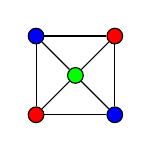
\begin{tikzpicture}
	\begin{scope}[every node/.style={circle, draw, inner sep = 2pt}]
	    	\node[fill=red] (1) at (0,0) {};
		\node[fill=blue] (2) at (0,1) {};
	    	\node[fill=red] (3) at (1,1) {};
		\node[fill=blue] (4) at (1,0) {};
		\node[fill=green] (5) at (0.5,0.5) {};
	\end{scope}
	
	\begin{scope}[>={Stealth[black]},
	              every node/.style={fill=white,circle},
	              every edge/.style={draw=black}]
		\path (1) edge (2);
		\path (2) edge (3);
		\path (3) edge (4);
		\path (4) edge (1);
		\foreach \i in {1,2,3,4} {\path (5) edge (\i);}
	\end{scope}
	\end{tikzpicture}
	\ee

% 3
\item Suppose a graph $G$ has chromatic number 1. What can you say about $G$?\\
	There are no edges in G.

% 4
\item 
	\be
	% 4 a
	\item Use the greedy algorithm to color the graph $G$ in Figure 2. How many colors did you use? I used \textbf{5} colors.
	\vspace{0.5cm}\\
	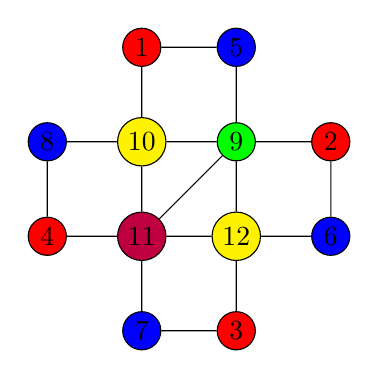
\begin{tikzpicture}[every node/.style={draw, circle, inner sep = 2 pt}, scale=1.2]
	\node[fill=red] (1) at (0,2) {1};
	\node[fill=red] (2) at (2,1) {2};
	\node[fill=red] (3) at (1,-1) {3};
	\node[fill=red] (4) at (-1,0) {4};
	\node[fill=blue] (5) at (1,2) {5};
	\node[fill=blue] (6) at (2,0) {6};
	\node[fill=blue] (7) at (0,-1) {7};
	\node[fill=blue] (8) at (-1,1) {8};
	\node[fill=green] (9) at (1,1) {9};
	\node[fill=yellow] (10) at (0,1) {10};
	\node[fill=purple] (11) at (0,0) {11};
	\node[fill=yellow] (12) at (1,0) {12};
	\draw (10) -- (1) -- (5) -- (9) -- (2) -- (6) -- (12) -- (3) -- (7) -- (11) -- 
		 (4) -- (8) -- (10) -- (9) -- (12) -- (11) -- (10) (11) --(9);
	\end{tikzpicture}
	% 4 b
	\item Determine the chromatic number of $G$. Justify that the number you find really is the number of colors needed.\\
	$\chi(G)=3$. This is the smallest possible chromatic number because there is an odd cycle. \vspace{0.5cm}\\
	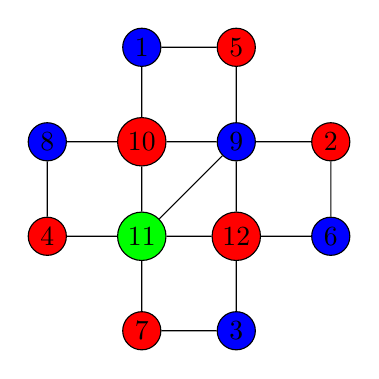
\begin{tikzpicture}[every node/.style={draw, circle, inner sep = 2 pt}, scale=1.2]
	\node[fill=blue] (1) at (0,2) {1};
	\node[fill=red] (2) at (2,1) {2};
	\node[fill=blue] (3) at (1,-1) {3};
	\node[fill=red] (4) at (-1,0) {4};
	\node[fill=red] (5) at (1,2) {5};
	\node[fill=blue] (6) at (2,0) {6};
	\node[fill=red] (7) at (0,-1) {7};
	\node[fill=blue] (8) at (-1,1) {8};
	\node[fill=blue] (9) at (1,1) {9};
	\node[fill=red] (10) at (0,1) {10};
	\node[fill=green] (11) at (0,0) {11};
	\node[fill=red] (12) at (1,0) {12};
	\draw (10) -- (1) -- (5) -- (9) -- (2) -- (6) -- (12) -- (3) -- (7) -- (11) -- 
		 (4) -- (8) -- (10) -- (9) -- (12) -- (11) -- (10) (11) --(9);
	\end{tikzpicture}
	\ee

% 5
\item
The math department is trying to schedule focus group interviews with students for certain classes outside of the ordinary class time. The courses have the following (entirely made up) student overlaps:\\
\begin{tabular}{c| c |c| c| c|c|c}
& Math 265 & Math 314 & Math 307 & Math 490 & Math  405 & Math 422 \\
\hline
Math 265 &  & 1 &  5 & 0 & 0&2\\ \hline
Math 314 & 1 &  & 0 & 0 & 0 & 0\\	\hline
Math 307 & 5 & 0 & & 1 & 0 & 2\\	\hline
Math 490 & 0 & 0 & 1&   &4& 2 \\ 	\hline
Math 405 & 0 & 0 & 0 & 4 & & 4 \\ \hline
Math 422 &2 & 0 & 2 & 2 &  4 & \\
\hline
\end{tabular}

	\be
	% 5 a
	\item Construct a graph representing the student overlaps (that is, assign the vertices to be the classes, and connect the 
	vertices with an edge if there are students in both classes, labelled with the number of students in both classes).\\
	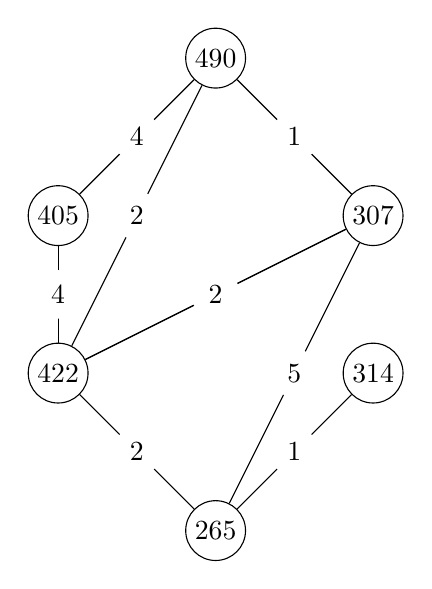
\begin{tikzpicture}
	\begin{scope}[every node/.style={circle, draw, inner sep = 2pt}]
	    	\node (265) at (0,0) {265};
	    	\node (314) at (2,2) {314};
	    	\node (307) at (2,4) {307};
	    	\node (490) at (0,6) {490};
	    	\node (405) at (-2,4) {405};
	    	\node (422) at (-2,2) {422};
	\end{scope}
	
	\begin{scope}[>={Stealth[black]},
	              every node/.style={fill=white,circle},
	              every edge/.style={draw=black}]
		\path (265) edge node{1} (314);
		\path (265) edge node{5} (307);
		\path (265) edge node{2} (422);
		\path (307) edge node{1} (490);
		\path (307) edge node{2} (422);
		\path (307) edge node{2} (422);
		\path (490) edge node{4} (405);
		\path (490) edge node{2} (422);
		\path (405) edge node{4} (422);
	\end{scope}
	\end{tikzpicture}
	% 5 b
	\item How many meeting times are needed? Explain, briefly.\\
	The number of meeting times is equal to $\chi(G)$. $\chi(G)$ of the graph below is 3, and $\chi(G)\geq3$, so there needs to 
	be at least 3 meetings.\vspace{0.5cm}\\
	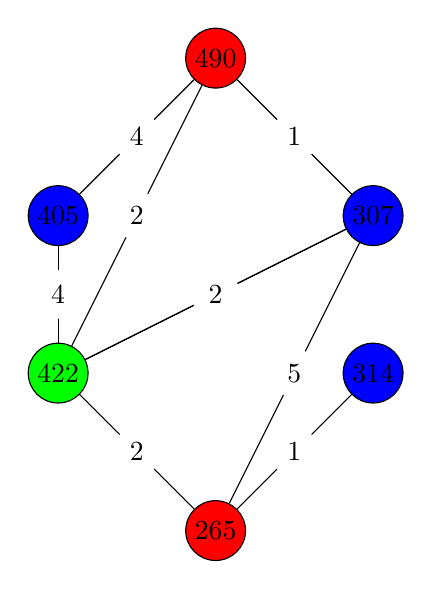
\begin{tikzpicture}
	\begin{scope}[every node/.style={circle, draw, inner sep = 2pt}]
	    	\node[fill=red] (265) at (0,0) {265};
	    	\node[fill=blue] (314) at (2,2) {314};
	    	\node[fill=blue] (307) at (2,4) {307};
	    	\node[fill=red] (490) at (0,6) {490};
	    	\node[fill=blue] (405) at (-2,4) {405};
	    	\node[fill=green] (422) at (-2,2) {422};
	\end{scope}
	
	\begin{scope}[>={Stealth[black]},
	              every node/.style={fill=white,circle},
	              every edge/.style={draw=black}]
		\path (265) edge node{1} (314);
		\path (265) edge node{5} (307);
		\path (265) edge node{2} (422);
		\path (307) edge node{1} (490);
		\path (307) edge node{2} (422);
		\path (307) edge node{2} (422);
		\path (490) edge node{4} (405);
		\path (490) edge node{2} (422);
		\path (405) edge node{4} (422);
	\end{scope}
	\end{tikzpicture}
	% 5 c
	\item Suppose only three meeting times are available, at 9AM, 10AM and 11AM, and furthermore, suppose that only one class is 
	allowed to meet at 9AM.  Is it possible to schedule the focus groups with this restriction? If so, give a possible schedule. 
	If not, explain why not.
		\begin{itemize}
		\item 9 AM: 422
		\item 10 AM: 405, 307, 314
		\item 11 AM: 490, 265
		\end{itemize}
	\ee

% 6
\item There are seven tour bus companies in the Los Angeles Area. During a particular day, each visits at most three locations from among Hollywood, Beverly Hills, Disneyland, and Universal Studios. The same location cannot be visited by more than one company on the same day. The first tour company visits only Hollywood, the second only Hollywood and Disneyland, the third only Universal Studios, the fourth only Disneyland and Universal Studios, the fifth Hollywood and Beverly Hills, the sixth Beverly Hills and Universal Studios, and the seventh Disneyland and Beverly Hills. Can these tours be scheduled only on Monday, Wednesday and Friday? Support/explain your answer.
	\begin{itemize}
	\item Monday: 7th company
	\item Wednesday: 2nd, 3rd, 5th companies
	\item Friday: 1st, 6th, 4th companies
	\end{itemize}
	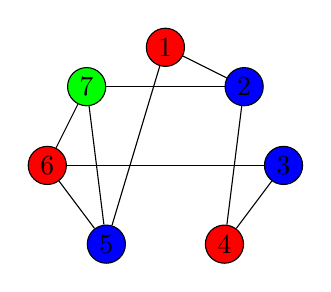
\begin{tikzpicture}
	\begin{scope}[every node/.style={circle, draw, inner sep = 2pt}]
	    	\node[fill=red] (1) at (0,0) {1};
		\node[fill=blue] (2) at (1,-0.5) {2};
	    	\node[fill=blue] (3) at (1.5,-1.5) {3};
		\node[fill=red] (4) at (0.75,-2.5) {4};
	    	\node[fill=blue] (5) at (-0.75,-2.5) {5};
	    	\node[fill=red] (6) at (-1.5,-1.5) {6};
		\node[fill=green] (7) at (-1,-0.5) {7};
	\end{scope}
	
	\begin{scope}[>={Stealth[black]},
	              every node/.style={fill=white,circle},
	              every edge/.style={draw=black}]
		\path (1) edge (2);
		\path (1) edge (5);
		\path (2) edge (4);
		\path (2) edge (7);
		\path (3) edge (4);
		\path (3) edge (6);
		\path (5) edge (6);
		\path (5) edge (7);
		\path (6) edge (7);
	\end{scope}
	\end{tikzpicture}

% 7
\item Prove that the Gr\"otzsch graph $G_{5}$, shown in Figure 3a, has $\chi(G) = 4$ by doing the following:
	\be
	% 7 a
	\item Find a 4-coloring of $G$. \vspace{0.5cm}\\
	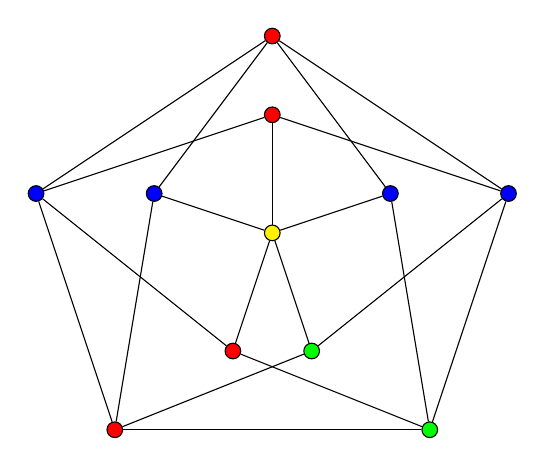
\begin{tikzpicture}
	\begin{scope}[every node/.style={circle, draw, inner sep = 2pt}]
	    	\node[fill=red] (1) at (0,0) {};
		\node[fill=blue] (2) at (-1,3) {};
	    	\node[fill=red] (3) at (2,5) {};
		\node[fill=blue] (4) at (5,3) {};
	    	\node[fill=green] (5) at (4,0) {};
	    	\node[fill=red] (6) at (2,4) {};
	    	\node[fill=blue] (7) at (3.5,3) {};
	    	\node[fill=green] (8) at (2.5,1) {};
	    	\node[fill=red] (9) at (1.5,1) {};
	    	\node[fill=blue] (10) at (0.5,3) {};
	    	\node[fill=yellow] (11) at (2,2.5) {};
	\end{scope}
	
	\begin{scope}[>={Stealth[black]},
	              every node/.style={fill=white,circle},
	              every edge/.style={draw=black}]
		\path (1) edge (2);
		\path (1) edge (5);
		\path (2) edge (3);
		\path (3) edge (4);
		\path (4) edge (5);
		\path (1) edge (10);
		\path (1) edge (8);
		\path (2) edge (6);
		\path (2) edge (9);
		\path (3) edge (10);
		\path (3) edge (7);
		\path (4) edge (6);
		\path (4) edge (8);
		\path (5) edge (7);
		\path (5) edge (9);
		\foreach \i in {6,7,8,9,10}{\path (11) edge (\i);}
	\end{scope}
	\end{tikzpicture}
	% 7 b
	\item Suppose that $G$ has a 3-coloring, say using red, green, blue. Without loss of generality, we may suppose the center 
	vertex is colored red. Explain why this forces a contradiction.\\
	The vertices around the center vertex create an odd number cycle, so they must be colored with at least 3 different colors. 
	The center vertex connects to all of these vertices, so it has to be a different color. That makes the chromatic number at 
	least 4. Thus $G$ cannot have a 3-coloring.
	% 7 c
	\item The Gr\"otzsch graph is a member of an infinite family of triangle-free graphs, . The graph $G_{6}$ is shown in Figures 
	3b. What is $\chi(G_{6})$? \\
	$\chi(G)=3$\vspace{0.5cm} \\
	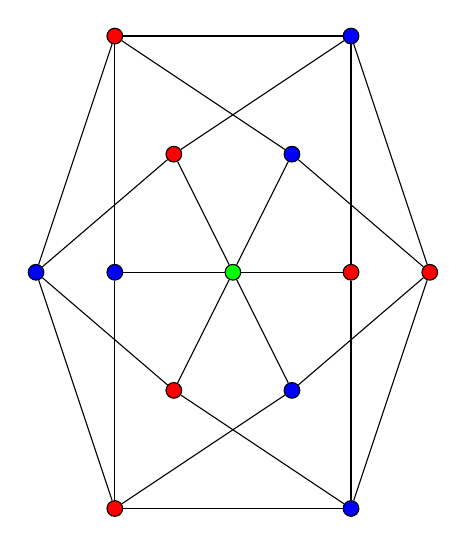
\begin{tikzpicture}
	\begin{scope}[every node/.style={circle, draw, inner sep = 2pt}]
	    	\node[fill=red] (1) at (0,0) {};
		\node[fill=blue] (2) at (-1,3) {};
	    	\node[fill=red] (3) at (0,6) {};
		\node[fill=blue] (4) at (3,6) {};
	    	\node[fill=red] (5) at (4,3) {};
	    	\node[fill=blue] (6) at (3,0) {};
	    	\node[fill=red] (7) at (0.75,4.5) {};
	    	\node[fill=blue] (8) at (2.25,4.5) {};
	    	\node[fill=red] (9) at (3,3) {};
	    	\node[fill=blue] (10) at (2.25,1.5) {};
	    	\node[fill=red] (11) at (0.75,1.5) {};
	    	\node[fill=blue] (12) at (0,3) {};
	    	\node[fill=green] (13) at (1.5,3) {};
	\end{scope}
	
	\begin{scope}[>={Stealth[black]},
	              every node/.style={fill=white,circle},
	              every edge/.style={draw=black}]
		\path (1) edge (2);
		\path (1) edge (10);
		\path (1) edge (12);
		\path (1) edge (6);
		\path (2) edge (3);
		\path (2) edge (7);
		\path (2) edge (11);
		\path (3) edge (12);
		\path (3) edge (8);
		\path (3) edge (4);
		\path (4) edge (7);
		\path (4) edge (9);
		\path (4) edge (5);
		\path (5) edge (6);
		\path (5) edge (10);
		\path (5) edge (8);
		\path (6) edge (11);
		\path (6) edge (9);
		\foreach \i in {7,8,9,10,11,12}{\path (13) edge (\i);}
	\end{scope}
	\end{tikzpicture}
	\ee

\ee

\end{document}















